% file: chap4.tex

\chapter{神经网络可以计算任何函数的可视化证明}
\label{ch:VisualProof}

神经网络的一个最显著的事实就是它可以计算任何的函数。也就是说,假设某个人给你某种
复杂而奇特的函数,$f(x)$:
\begin{center}
  \includegraphics{function}
\end{center}

\label{basic_network_precursor}不管这个函数是什么样的,总会确保有一个神经网络能够
对任何可能的输入 $x$,其值 $f(x)$ (或者某个足够准确的近似)是网络的输出,例如:
\begin{center}
  \includegraphics{basic_network}
\end{center}

即使函数有很多输入和输出,$f = f(x_1, \ldots, x_m)$,这个结果都是成立的。例如,这
个网络计算一个具有 $m = 3$ 个输入和 $n = 2$ 个输出的函数:
\begin{center}
  \includegraphics{vector_valued_network}
\end{center}

结果表明神经网络拥有一种\textbf{普遍性}。不论我们想要计算什么样的函数,我们都确信存
在一个神经网络可以计算它。

而且,这个普遍性定理甚至在我们限制了神经网络只在输入层和输出层之间存在一个中间层
的情况下成立。所以即使是很简单的网络架构都极其强大。

普遍性定理在使用神经网络的人群中是众所周知的。但是它为何正确却不被广泛地理解。现
有的大多数的解释都具有很强的技术性。例如,有一篇原始的论
文\footnote{\href{http://www.dartmouth.edu/~gvc/Cybenko_MCSS.pdf}{Approximation
    by superpositions of a sigmoidal function},作者为 George Cybenko (1989)。其
  结论在当时非常流行,并且几个研究小组证明了密切相关的结果。Cybenko 的论文包含了
  很多关于那些成果非常有用的讨论。另一篇重要的早期论文是
  \href{http://www.sciencedirect.com/science/article/pii/0893608089900208}{Multilayer
    feedforward networks are universal approximators},作者为 Kurt Hornik,
  Maxwell Stinchcombe,和 Halbert White (1989)。这篇论文采用了 Stone-Weierstrass
  定理来取得相似的结果。}使用了\href{https://zh.wikipedia.org/wiki/哈恩-巴拿赫
  定理}{哈恩-巴拿赫定理定理}、\href{https://zh.wikipedia.org/wiki/里斯表示定理}{里
  斯表示定理}和一些傅里叶分析证明了这个结果。如果你是数学家,这个证明应该不大难
理解,但对于大多数人还是很困难的。这不得不算是一种遗憾,因为这个普遍性背后的原理
其实是简单而美妙的。

在这一章,我给出这个普遍性定理的简单且大部分为可视化的解释。我们会一步步深入背后
的思想。你会理解为何神经网络可以计算任何的函数。你会理解到这个结论的一些局限。并
且你还会理解这些结论如何和深度神经网络关联的。

要跟随本章的内容,你不需要读过本书前面的章节。相反,本章其实可以当成独立的短文阅
读。如果你已经对神经网络有了一点基本的了解,你应该能够弄清楚这些解释。然而,我偶
尔也会给出一些联系到前面的章节的链接,帮助你填补一些知识结构的空白。

普遍性定理在计算机科学领域中常常会有,太多了以至于我们有时候都忘了这些定理的特别
之处。但值得提醒自己的是:计算任意函数的能力真是太赞了。几乎你可以想象的任何过程
都可以看做是函数的计算。考虑给一段音乐用短的音乐片段进行命名这个问题。这其实也能
够看做是计算一个函数。或者考虑将中文文本翻译成英文。同样,这又可以看成是计算一个
函数\footnote{实际上可以看成是计算很多的函数,因为对于一段文本来说有很多种翻译。}。
又或者根据一个 mp4 视频文件生成一个描述电影情节并讨论表演质量的问题。同样,这些也
都可以看成是一种类型的函数计算\footnote{同上,关于翻译和有多种可能的函数的注释。}。
普遍性是指,在原理上,神经网络可以做所有这些事情,或者更多。

当然,仅仅因为我们知道存在一个可以将中文翻译成英文的神经网络,这并不意味着我们有
了一种构造甚至识别出这样的网络的很好的技术。这个局限同样可以应用在诸如布尔电路上
的传统的普遍性定理上。但是,如同我们在前文看到的那样,神经网络拥有强大的算法来学
习函数。学习算法和普遍性的结合是一种有趣的混合。直到现在,本书一直是着重谈学习算
法。到了本章,我们来看看普遍性,看看它究竟意味着什么。

\section{两个预先声明}
\label{sec:two_caveats}

在解释为何普遍性定理成立前,我想要提下关于非正式的表述“神经网络可以计算任何函
数”的两个预先声明。

第一点,这句话不是说一个网络可以被用来\textbf{准确地}计算任何函数。而是说,我们可以
获得尽可能好的一个\textbf{近似}。通过增加隐藏元的数量,我们可以提升近似的精度。例
如,\hyperref[basic_network_precursor]{前面}我举例说明一个使用了三个隐藏元的网络
来计算 $f(x)$。对于大多数函数使用三个隐藏元仅仅能得到一个低质量的近似。通过增加隐
藏神经元的数量(比如说,五个),我们能够明显地得到更好的近似:
\begin{center}
  \includegraphics{bigger_network}
\end{center}

并且我们可以继续增加隐藏神经元的数目。

为了让这个表述更加准确,假设我们给定一个需要按照目标精度 $\epsilon > 0$ 的函数
$f(x)$。通过使用足够多的隐藏神经元使得神经网络的输出 $g(x)$ 对所有的 $x$,满足
$|g(x) - f(x)| < \epsilon$ 从而实现近似计算。换言之,近似对每个可能的输入都是限
制在目标准确度范围内的。

第二点,就是可以按照上面的方式近似的函数类其实是\textbf{连续}函数。如果函数不是连
续的,也就是会有突然、极陡的跳跃,那么一般来说无法使用一个神经网络进行近似。这并
不意外,因为神经网络计算的就是输入的连续函数。然而,即使那些我们真的想要计算的函
数是不连续的,一般来说连续的近似其实也足够的好了。如果这样的话,我们就可以用神经
网络来近似了。实践中,这通常不是一个严重的限制。

总结一下,更加准确的关于普遍性定理的表述是包含一个隐藏层的神经网络可以被用来按照
任意给定的精度来近似任何连续函数。本章,我们会使用了两个隐藏层的网络来证明这个结
果的弱化版本。在问题中我将简要介绍如何通过一些微调把这个解释适应于只使用一个隐藏
层的网络的证明。

\section{一个输入和一个输出的普遍性}
\label{sec:universality_with_one_input_and_one_output}

为了理解为何普遍性定理成立,我们先从理解如何构造这样一个神经网络开始,它能够近似
一个只有一个输入和一个输出的函数:
\begin{center}
  \includegraphics{function}
\end{center}

结果表明,这其实是普遍性问题的核心。一旦我们理解了这个特例,那么实际上就会很容易
扩展到那些有多个输入输出的函数上。

为了构建关于如何构造一个计算 $f$ 的网络的理解,让我们从一个只包含一个隐藏层的网
络开始,它有两个隐藏神经元,和单个输出神经元的输出层:
\begin{center}
  \includegraphics{two_hidden_neurons}
\end{center}

为了感受一下网络的组成部分工作的机制,我们专注于最顶上的那个隐藏神经元。在下图例
子中,展示了顶部隐藏神经元的权重 $w$,偏置 $b$ 和输出曲线的关系。思考最上面的隐
藏神经元变化如何计算函数:
\begin{center}
  \includegraphics{basic_manipulation}
\end{center}

正如我们在\hyperref[sec:sigmoid_neurons]{本书前面}学到的,隐藏神经元在计算的
是 $\sigma(wx + b)$,这里 $\sigma(z) \equiv 1/(1+e^{-z})$ 是 S 型函数。目前为止,
我们已经频繁使用了这个代数形式。但是为了证明普遍性,我们会完全忽略其代数性质,取
而代之的是在图形中调整和观察形状来获取更多的领悟。这不仅会给我们更好的感性认识,
而且它也会给我们一个可应用于除了S型函数之外其它激活函数的普遍性的证明\footnote{严
  格地说,我所采取的可视化方式传统上并不被认为是一个证明。但我相信可视化的方法比
  一个传统的证明能给出更深入的了解。当然,这种了解是证明背后的真正目的。偶尔,在
  我呈现的推理中会有小的差距:那些有可视化参数的地方,看上去合理,但不是很严谨。
  如果这让你烦恼,那就把它视为一个挑战,来填补这些缺失的步骤。但不要忽视了真正的
  目的:了解为什么普遍性定理是正确的。}。

开始,增加偏置 $b$ 的值。当偏置增加时,图形往左移动,但是形状不变。

接下来,减小偏置。当偏置减小时图形往右移动,但是再一次,它的形状没有变化。

继续,将权重减小到大约 $2$ 或 $3$。当你减小权重时,曲线往两边拉宽了。你可以同时
改变偏置,让曲线保持在框内。

最后,把权重增加到超过 $w = 100$。当你这样做时,曲线变得越来越陡,直到最终看上去
就像是一个阶跃函数。试着调整偏置,使得阶跃位置靠近 $x = 0.3$。下面一个图示显示你
应该看到的结果。
\begin{center}
  \includegraphics{create_step_function}
\end{center}

你能给权重增加很大的值来简化我们的分析,使得输出实际上是个非常接近的阶跃函数。下
面我画出了当权重为 $w = 999$ 时从顶部隐藏神经元的输出。
\begin{center}
  \includegraphics{high_weight_function}
\end{center}

实际上处理阶跃函数比一般的 S 型函数更加容易。原因是在输出层我们把所有隐藏神经元的
贡献值加在一起。分析一串阶跃函数的和是容易的,相反,思考把一串 S 形状的曲线加起来
是什么则要更困难些。所以假设我们的隐藏神经元输出阶跃函数会使事情更容易。更具体些,
我们把权重 $w$ 固定在一个大的值,然后通过修改偏置设置阶跃函数的位置。当然,把输出
作为一个阶跃函数处理只是一个近似,但是它是一个非常好的近似,现在我们把它看作是精
确的。稍后我会再讨论偏离这种近似的影响。

$x$ 取何值时阶跃会发生呢?换种方式,阶跃的位置如何取决于权重和偏置?

为了回答这个问题,试着修改上面图中的权重和偏置(你可能需要向上滚动一点)。你能不
能算出阶跃的位置如何取决于 $w$ 和 $b$?做点工作你应该能够说服自己,阶跃的位置
和 $b$ \textbf{成正比},和 $w$ \textbf{成反比}。

实际上,阶跃发生在 $s = -b/w$ 的位置,正如你能在下图中通过修改权重和偏置看到的:
\begin{center}
  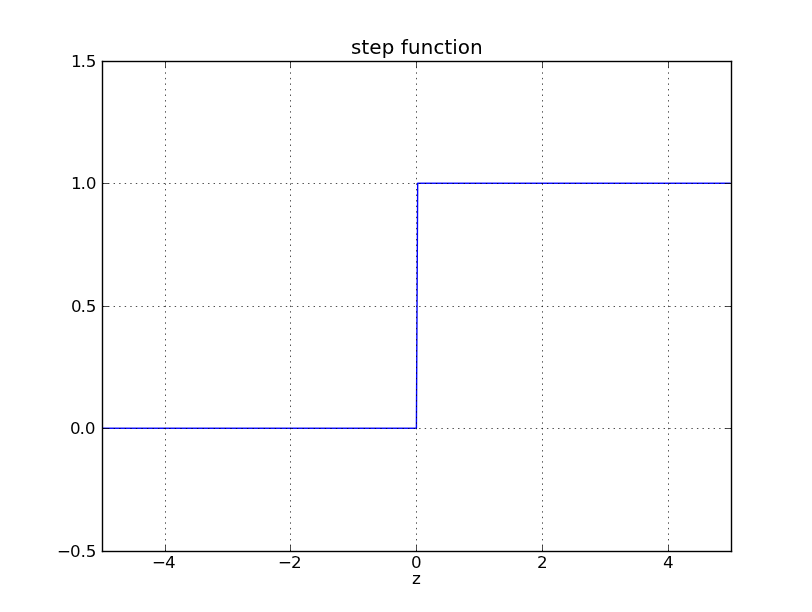
\includegraphics{step}
\end{center}

这将用仅仅一个参数 $s$ 来极大简化我们描述隐藏神经元的方式,这就是阶跃位置,$s =
-b/w$。试着修改下图中的 $s$,以便习惯这个新的参数设定:
\begin{center}
  \includegraphics{step_parameterization}
\end{center}

正如上面注意到的,我们隐式地设置输入上的权重 $w$ 为一些大的值~——~大到阶跃函数能够
很好地近似。通过选择偏置 $b = -ws$,我们能很容易地将一个以这种方式参数化的神经元
转换回常用的模型。

目前为止我们专注于仅仅从顶部隐藏神经元输出。让我们看看整个网络的行为。尤其,我们
假设隐藏神经元在计算以阶跃点 $s_1$ (顶部神经元)和 $s_2$ (底部神经元)参数化的
节约函数。它们各自有输出权重 $w_1$ 和 $w_2$。是这样的网络:
\begin{center}
  \includegraphics{two_hn_network}
\end{center}

右边的绘图是隐藏层的\textbf{加权输出} $w_1 a_1 + w_2 a_2$。这里 $a_1$ 和 $a_2$ 各自
是顶部和底部神经元的输出\footnote{顺便提一下,注意整个网络的输出是 $\sigma(w_1
  a_1+w_2 a_2 + b)$,其中 $b$ 是隐藏层的偏置。很明显,这不同于隐藏层加权后的输出,
  也就是我们这里的绘图。我们现在打算专注于隐藏层的加权输出,不一会就会考虑如何把
  它关联到整个网络的输出。}。这些输出由 $a$ 表示,是因为它们通常被称为神经元
的\textbf{激活值}(\textbf{activations})。

试着增加和减小顶部隐藏神经元的阶跃点 $s_1$。感受下这如何改变隐藏层的加权输出。尤
其值得去理解当 $s_1$ 经过 $s_2$ 时发生了什么。你会看到这时图形发生了变化,因为我
们从顶部隐藏神经元先被激活的情况变成了底部隐藏神经元先被激活的情况。

类似地,试着操作底部隐藏神经元的阶跃点 $s_2$,感受下这如何改变隐藏神经元混合后的
输出。

尝试增加和减少每一个输出权重。注意,这如何调整从各自的隐藏神经元的贡献值。当一个
权重是 0 时会发生什么?

最后,试着设置 $w_1$ 为 $0.8$,$w_2$ 为 $-0.8$。你得到一个“凸起”的函数,它从
点 $s_1$ 开始,到点 $s_2$ 结束,高为 $0.8$。例如,加权后的输出可能看起来像这样:
\begin{center}
  \includegraphics{bump_function}
\end{center}

当然,我们可以调整为任意的凸起高度。让我们用一个参数,$h$,来表示高度。为了减少混
乱我也会移除“$s_1 = \ldots$”和“$w_1 = \ldots$”的标记。
\begin{center}
  \includegraphics{bump_fn}
\end{center}

试着将 $h$ 值改大或改小,看看凸起的高度如何改变。试着把高度值改为负数,观察发生了
什么。并且试着改变阶跃点来看看如何改变凸起的形状。

顺便提一下,你会注意到,我们用神经元的方式,可以认为不只是在图形的角度,而且是更
传统的编程形式,作为 {\serif if-then-else} 的一种声明,即:
\begin{lstlisting}[language=Python]
    if input >= step point:
        add 1 to the weighted output
    else:
        add 0 to the weighted output  
\end{lstlisting}

对于大部分内容,我将坚持以图形的考虑角度。但在接下来的内容中,你有时可能会发现交
换考虑角度是有帮助的,并且考虑 {\serif if-then-else} 的形式。

我们可以用凸起制作的技巧来得到两个凸起,通过把两对隐藏神经元一起填充进同一个网
络:
\begin{center}
  \includegraphics{double_bump}
\end{center}

这里我抑制了权重,只是简单地在每对隐藏神经元上写了 $h$ 的值。试着增加和减少两
个 $h$ 值,观察它如何改变图形。通过修改节点来移动凸起。

更普遍地,我们可以利用这个思想来取得我们想要的任何高度的峰值。尤其,我们可以把间
隔 $[0, 1]$分成大量的子区间,用 $N$ 表示,并利用 $N$ 对隐藏神经元来设置任意期望高
度的峰值。让我们看看 $N = 5$ 这如何工作。那样确实有很多神经元,所以我打算弄得挤一
些。抱歉这个图示有些复杂:我能通过更进一步的抽象来隐藏其复杂性,但是我想多些复杂
是值得的,为了获得网络如何工作的更具体的感受。
\begin{center}
  \includegraphics{five_bumps}
\end{center}
你能看到有五对隐藏神经元。每对神经元对应的连接点是 $0, 1/5$,然后是 $1/5, 2/5$等
等,最后到 $4/5, 5/5$。这些值是固定的 -- 它们使得我们在图形上得到五个均匀分布的
凸起。

每对神经元有一个值 $h$ 和它联系。记住,神经元输出的连接有权重 $h$ 和 $-h$ (未标
记)。点击一个 $h$ 值,左右拖动鼠标来改变其值。当你这么做的时候,观察函数的变化。
通过改变输出权重我们实际上在\textbf{设计}这个函数。

相反地,试着在图形上点击,上下拖动来改变凸起函数的高度。当你改变高度,你能看到相
应的 $h$ 值的变化。而且,虽然没有显示,在对应的输出权重上也有一个变
化,$+h$ 和$-h$。

换句话说,我们可以直接操作右边图形里的函数,然后看看反映到左边的 $h$ 值。一个有趣
的事情是按住鼠标按键并从图形的一边拖动到另一边。这样做你拉出了一个函数,观察神经
网络中为了适应这个函数调整的参数。

是时候来个挑战了。

让我们回想我在本章开始绘制出的函数:
\begin{center}
  \includegraphics{function}
\end{center}

那时我没有说,但是我绘制的其实是函数
\begin{equation}
f(x) = 0.2+0.4 x^2+0.3x \sin(15 x) + 0.05 \cos(50 x)
\label{eq:113}\tag{113}
\end{equation}
$x$ 取值范围从 $0$ 到 $1$,$y$ 轴取值为 $0$ 到 $1$。

它明显不是一个微不足道的函数。

你将要解出如何使用一个神经网络来计算它。

在我们上面的网络中,我们已经分析了隐藏神经元输出的加权组合
$\sum_j w_j a_j$。我们现在知道如何在这个量上获得大量的控制。但是,正如我前面所指
出的,这个量不是网络的输出。网络输出的是 $\sigma(\sum_j w_j a_j + b)$,其中 $b$
是在输出神经元的偏置。有什么办法可以实现对网络的实际输出控制吗?

解决方案是设计一个神经网络,它的隐藏层有一个加权输出 $\sigma^{-1} \circ f(x)$,其
中 $\sigma^{-1}$是 $\sigma$ 函数的反函数。也就是说,我们希望从隐藏层的加权输出是:
\begin{center}
  \includegraphics{inverted_function}
\end{center}

如果你能这样做,那么整体来看网络的输出会是 $f(x)$ 的一个很好的近似\footnote{注意
  我已经将输出神经元上的偏置设置为 $0$。}。

那么你的挑战,是在%
\href{http://neuralnetworksanddeeplearning.com/chap4.html#universality_with_one_input_and_one_output}{%
  网页}上设计一个神经网络可近似上面显示的目标函数。为了尽可能多地学习,我希望你
能分两次解决这个问题。第一次,请在图形上点击,直接调整不同的凹凸函数的高度。你应
该能发现找到一个很好的匹配的目标函数是很容易的。你做的有多好通过目标函数和网络实
际计算函数的\textbf{平均偏差}来衡量。你的挑战是尽可能\textbf{低}的平均偏差。当你将平
均偏差争取到 $0.40$ 或以下时,你完成了挑战。

一旦你完成了,点击“重置”,随机重新初始化凹凸形状。你第二次解决问题时,忍住在图
形上点击的冲动。相反,修改左边的 $h$ 值,并再次尝试将平均偏差争取到 $0.40$ 或以
下。点击下面的图形可链接到网页并开始你的设计。
\begin{center}
  \href{http://neuralnetworksanddeeplearning.com/chap4.html#universality_with_one_input_and_one_output}{\includegraphics{design_function}}
\end{center}

一个完成的图形看起来像是这样:
\begin{center}
  \includegraphics{design_function_success}
\end{center}

你现在已经解决了所有网络的必要元素来近似计算函数 $f(x)$!这只是一个粗略的近似,
但我们可以很容易地做得更好,仅仅通过增加隐藏神经元对的数量,分配更多的凹凸形状。

特别是,将我们已经找到的所有数据转换回神经网络使用的标准参数设定是很容易的。让我
快速总结一下那是如何工作的。

第一层的权重都有一些大的,恒定的值,比如:$w = 1000$。

隐藏神经元上的偏置只是 $b = -w s$。例如,对于第二个隐藏神经元 $s = 0.2$ 变成了
$b = -1000 \times 0.2 = -200$。

最后一层的权重由 $h$ 值决定。例如,我们上面已经选择的第一个 $h$,$h = -0.5$,意
味着顶部两个隐藏神经元的相应的输出权重是 $-0.5$ 和 $0.5$。如此等等,确定整个层的
输出权重。

最后,输出神经元的偏置为 $0$。

这是所有要做的事情:现在我们有了一个可以很好计算我们原始目标函数的神经网络的完整
的描述。而且我们理解如何通过提高隐层神经元的数目来提高近似的质量。

更重要的是,关于我们的原始目标函数 $f(x) = 0.2+0.4 x^2+0.3 \sin(15 x) + 0.05
\cos(50 x)$,没有什么特别的。我们可以用这个程序计算任何定义域为 $[0, 1]$,值域为
$[0, 1]$ 的连续函数。在本质上,我们使用我们的单层神经网络来建立一个函数的查找表。
我们将能够建立这个思想,以提供普遍性的一般性证明。

\section{多个输入变量}
\label{sec:many_input_variables}

让我们把结果扩展到有很多个输入变量的情况下。这听上去挺复杂,但是所有我们需要的概
念都可以在两个输入的情况下被理解。所以让我们处理两个输入的情况。

我们从考虑当一个神经元有两个输入会发生什么开始:
\begin{center}
  \includegraphics{two_inputs}
\end{center}

这里,我们有输入 $x$ 和 $y$,分别对应于权重 $w_1$ 和 $w_2$,以及一个神经元上的偏
置 $b$。让我们把权重 $w_2$ 设置为 $0$,然后反复琢磨第一个权重 $w_1$ 和偏置 $b$,
看看他们如何影响神经元的输出:
\begin{center}
  \includegraphics{ti_graph}
\end{center}

正如你能看到的,在 $w_2 = 0$ 时输入 $y$ 对神经元的输出没有影响。它就像 $x$ 是唯
一的输入。

鉴于此,你认为当我们增加权重 $w_1$ 到 $w_1 = 100$,同时 $w_2$ 保持 $0$ 不变时会
发生什么?如果你没有立即明白答案,思考一下问题,看看你能否知道会发生什么。然后尝
试一下,看看你是否是对的。下面的图形序列展示了会发生什么:
\begin{center}
  \begin{tabular}{c c}
  \includegraphics{ti_graph-0} & \includegraphics{ti_graph-1}\\
  \includegraphics{ti_graph-2} & \includegraphics{ti_graph-3}\\
  \includegraphics{ti_graph-4} & \\
  \end{tabular}
\end{center}

正如我们前面讨论的那样,随着输入权重变大,输出接近一个阶跃函数。不同的是,现在的
阶跃函数是在三个维度。也如以前一样,我们可以通过改变偏置的位置来移动阶跃点的位置。
阶跃点的实际位置是 $s_x \equiv -b / w_1$。

让我们用阶跃点位置作为参数重绘上面的阶跃函数:
\begin{center}
  \includegraphics{ti_graph_redux}
\end{center}

这里,我们假设 $x$ 输入上的权重有一个大的值~——~我使用了 $w1 = 1000$~——~而权重
$w_2 = 0$。神经元上的数字是阶跃点,数字上面的小 $x$ 提醒我们阶跃在 $x$ 轴方向。
当然,通过使得 $y$ 输入上的权重取一个非常大的值(例如,$w_2 = 1000$),$x$ 上的
权重等于 $0$,即 $w_1 = 0$,来得到一个 $y$ 轴方向的阶跃函数也是可行的,
\begin{center}
  \includegraphics{y_step}
\end{center}

再一次,神经元上的数字是阶跃点,在这个情况下数字上的小 $y$ 提醒我们阶跃是在 $y$
轴方向。我本来可以明确把权重标记在 $x$ 和 $y$ 输入上,但是决定不这么做,因为这会
把图示弄得有些杂乱。但是记住小 $y$ 标记含蓄地告诉我们 $y$ 权重是个大的值,$x$ 权
重为 $0$。

我们可以用我们刚刚构造的阶跃函数来计算一个三维的凹凸函数。为此,我们使用两个神经
元,每个计算一个$x$ 方向的阶跃函数。然后我们用相应的权重 $h$ 和 $-h$ 将这两个阶
跃函数混合,这里 $h$ 是凸起的期望高度。所有这些在下面图示中说明:
\begin{center}
  \includegraphics{bump_3d}
\end{center}

试着改变高度 $h$ 的值。观察它如何和网络中的权重关联。并看看它如何改变右边凹凸函
数的高度。

另外,试着改变与顶部隐藏神经元相关的阶跃点 $0.30$。见证它如何改变凸起形状。当你
移动它超过和底部隐藏神经元相关的阶跃点 $0.70$ 时发生了什么?

我们已经解决了如何制造一个 $x$ 方向的凹凸函数。当然,我们可以很容易地制造一个
$y$ 方向的凹凸函数,通过使用 $y$ 方向的两个阶跃函数。回想一下,我们通过使 $y$输
入的权重变大,$x$ 输入的权重为 $0$ 来这样做。这是结果:
\begin{center}
  \includegraphics{bump_3d_y}
\end{center}

这看上去和前面的网络一模一样!唯一的明显改变的是在我们的隐藏神经元上现在标记有一
个小的 $y$。那提醒我们它们在产生 $y$ 方向的阶跃函数,不是 $x$ 方向的,并且 $y$上
输入的权重变得非常大,$x$ 上的输入为 $0$,而不是相反。正如前面,我决定不去明确显
示它,以避免图形杂乱。

让我们考虑当我们叠加两个凹凸函数时会发生什么,一个沿 $x$ 方向,另一个沿 $y$ 方向,
两者都有高度 $h$:
\begin{center}
  \includegraphics{xy_bump}
\end{center}

为了简化图形,我丢掉了权重为 $0$ 的连接。现在,我在隐藏神经元上留下了 $x$ 和 $y$
的标记,来提醒你凹凸函数在哪个方向上被计算。后面我们甚至为丢掉这些标记,因为它们
已经由输入变量说明了。

试着改变参数 $h$。正如你能看到,这引起输出权重的变化,以及 $x$ 和 $y$ 上凹凸函数
的高度。

我们构建的有点像是一个\textbf{塔型}函数:
\begin{center}
  \includegraphics{tower}
\end{center}

如果我们能构建这样的塔型函数,那么我们能使用它们来近似任意的函数,仅仅通过在不通
位置累加许多不同高度的塔:
\begin{center}
  \includegraphics{many_towers}
\end{center}

当然,我们还没有解决如何构建一个塔型函数。我们已经构建的看起来像一个中心塔,高度
为 $2h$,周围由高原包围,高度为 $h$。

但是我们能制造一个塔型函数。记得前面我们看到神经元能被用来实现一个 {\serif
  if-then-else} 的声明:
\begin{lstlisting}[language=Python]
    if input >= threshold: 
        output 1
    else:
        output 0
\end{lstlisting}

这是一个只有单个输入的神经元。我们想要的是将一个类似的想法应用到隐藏神经元的组合
输出:
\begin{lstlisting}[language=Python]
    if combined output from hidden neurons >= threshold:
        output 1
    else:
        output 0
\end{lstlisting}

如果我们选择适当的阈值~——~比如,$3h/2$,这是高原的高度和中央塔的高度中间的值 ——
我们可以把高原下降到零,并且依旧矗立着塔。

你能明白怎么做吗?试着用下面的网络做实验来解决。请注意,我们现在正在绘制整个网络
的输出,而不是只从隐藏层的加权输出。这意味着我们增加了一个偏置项到隐藏层的加权输
出,并应用 S 型函数。你能找到 $h$ 和 $b$ 的值,能产生一个塔型吗?这有点难,所以
如果你想了一会儿还是困住,这是有两个提示:(1)为了让输出神经元显示正确的{\serif
  if-then-else} 行为,我们需要输入的权重(所有 $h$ 或 $-h$)变得很大;(2)$b$
的值决定了 {\serif if-then-else} 阈值的大小。
\begin{center}
  \includegraphics{tower_construction}
\end{center}

在初始参数时,输出看起来像一个前面图形在它的塔型和高原上的平坦的版本。为了得到期
望的行为,我们增加参数 $h$ 直到它变得很大。这就给出了 {\serif if-then-else} 做阈
值的行为。其次,为了得到正确的阈值,我们选择 $b \approx -3h/2$。尝试一下,看看它
是如何工作的!

这是它看起来的样子,我们使用 $h = 10$:
\begin{center}
  \includegraphics{tower_construction_2}
\end{center}

甚至对于这个相对适中的 $h$ 值,我们得到了一个相当好的塔型函数。当然,我们可以通
过更进一步增加 $h$ 并保持偏置$b = -3h/2$ 来使它如我们所希望的那样。

让我们尝试将两个这样的网络组合在一起,来计算两个不同的塔型函数。为了使这两个子网
络更清楚,我把它们放在如下所示的分开的方形区域:每个方块计算一个塔型函数,使用上
面描述的技术。右边的图上显示了\textbf{第二个}隐藏层的加权输出,即,它是一个加权组
合的塔型函数。
\begin{center}
  \includegraphics{the_two_towers}
\end{center}

尤其你能看到通过修改最终层的权重能改变输出塔型的高度。

同样的想法可以用在计算我们想要的任意多的塔型。我们也可以让它们变得任意细,任意高。
结果,我们可以确保第二个隐藏层的加权输出近似与任意期望的二元函数:
\begin{center}
  \includegraphics{many_towers_2}
\end{center}

尤其通过使第二个隐藏层的加权输出为 $\sigma^{-1} \circ f$ 的近似,我们可以确保网
络的输出可以是任意期望函数 $f$ 的近似。

超过两个变量的函数会怎样?

让我们试试三个变量 $x_1, x_2, x_3$。下面的网络可以用来计算一个四维的塔型函数:
\begin{center}
  \includegraphics{tower_n_dim}
\end{center}

这里,$x_1, x_2, x_3$ 表示网络的输入。$s_1, t_1$ 等等是神经元的阶跃点~——~即,第
一层中所有的权重是很大的,而偏置被设置为给出阶跃点 $s_1, t_1, s_2, \ldots$。第二
层中的权重交替设置为 $+h, -h$,其中 $h$ 是一个非常大的数。输出偏置为 $-5h/2$。

这个网络计算这样一个函数,当三个条件满足时:$x_1$ 在 $s_1$ 和 $t_1$ 之间;$x_2$
在$s_2$ 和 $t_2$ 之间;$x_3$ 在 $s_3$ 和 $t_3$ 之间,输出为 $1$。其它情况网络输
出为 $0$。即,这个塔型在输入空间的一个小的区域输出为 $1$,其它情况输出 $0$。

通过组合许多个这样的网络我们能得到任意多的塔型,如此可近似一个任意的三元函数。对
于 $m$ 维可用完全相同的思想。唯一需要改变的是将输出偏置设为 $(-m+1/2)h$,为了得
到正确的夹在中间的行为来弄平高原。% 翻译成稳定平面?

好了,所以现在我们知道如何用神经网络来近似一个多元的实值函数。对于 $f(x_1,
\ldots, x_m) \in R^n$ 的向量函数怎么样?当然,这样一个函数可以被视为 $n$ 个单独
的实值函数: $f^1(x_1, \ldots, x_m)$, $f^2(x_1, \ldots, x_m)$ 等等。所以我们创
建一个网络来近似 $f^1$,另一个来近似 $f^2$,如此等等。然后简单地把这些网络都组合
起来。 所以这也很容易应付。

\subsection*{问题}

\begin{itemize}
  \item 我们已经看到如何使用具有两个隐藏层的网络来近似一个任意函数。你能否找到一
    个证明,证明只有一个隐藏层是可行的?作为一个提示,试着在只有两个输入变量的情
    况下工作,并证明:(a)可以得到一个不仅仅在 $x$ 和 $y$ 方向,而是在一个任意
    方向上的阶跃函数;(b)可以通过累加许多的源自(a)的结构,近似出一个塔型的函
    数,其形状是圆的,而不是方的;(c)使用这些圆形塔,可以近似一个任意函数。对
    于(c)可以使用\hyperref[sec:fixing_up_the_step_functions]{本章稍后}的一些思
    想。
\end{itemize}

\section{S 型神经元的延伸}
\label{sec:extension_beyond_sigmoid_neurons}

我们已经证明了由 S 型神经元构成的网络可以计算任何函数。回想下在一个 S 型神经元中,
输入$x_1, x_2, \ldots$ 导致输出 $\sigma(\sum_j w_j x_j + b)$,这里 $w_j$ 是权重,
$b$ 是偏置,而 $\sigma$ 是 S 型函数:
\begin{center}
  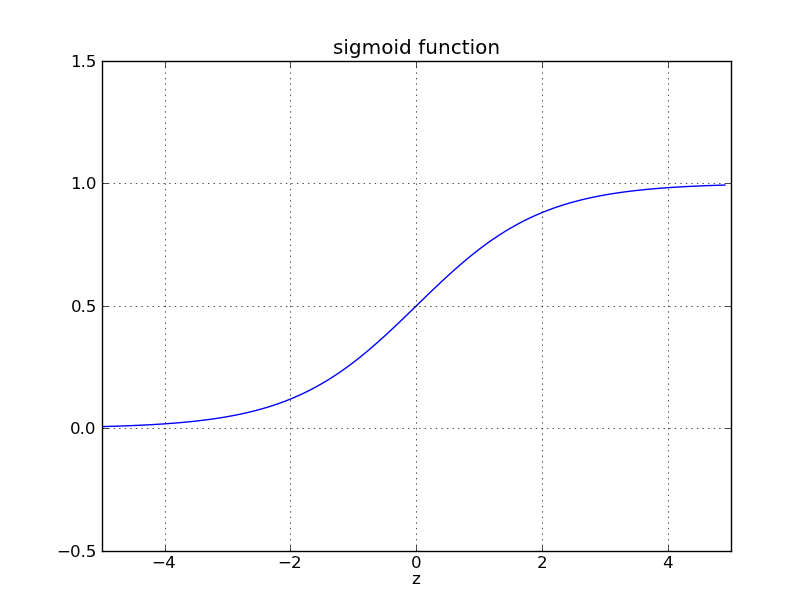
\includegraphics{sigmoid}
\end{center} 

如果我们考虑一个不同类型的神经元,它使用其它激活函数,比如如下的 $s(z)$,会怎样?
\begin{center}
  \includegraphics{sigmoid_like}
\end{center} 

更确切地说,我们假定如果神经元有输入 $x_1, x_2, \ldots$,权重 $w_1, w_2, \ldots$
和偏置 $b$,那么输出为 $s(\sum_j w_j x_j + b)$。我们可以使用这个激活函数来得到一
个阶跃函数,正如用 S 型函数做过的一样。
\begin{center}
  \includegraphics{ramping}
\end{center}

试着加大上图中的权重,比如 $w = 100$,你将得到:
\begin{center}
  \includegraphics{create_ramping}
\end{center}

正如使用 S 型函数的时候,这导致激活函数收缩,并最终变成一个阶跃函数的很好的近似。
试着改变偏置,然后你能看到我们可以设置我们想要的阶跃位置。所以我们能使用所有和前
面相同的技巧来计算任何期望的函数。

$s(z)$ 需要什么样的性质来满足这样的结果呢?我们确实需要假定 $s(z)$ 在 $z
\rightarrow -\infty$ 和 $z \rightarrow \infty$ 时是定义明确的。这两个界限是在我们
的阶跃函数上取的两个值。我们也需要假定这两个界限彼此不同。如果它们不是这样,就没
有阶跃,只是一个简单的平坦图形!但是如果激活函数 $s(z)$ 满足这些性质,基于这样一
个激活函数的神经元可普遍用于计算。

\subsection*{问题}

\begin{itemize}
\item 在本书前面我们遇到过其它类型的称为
  \hyperref[subsec:other_models_of_artificial_neuron]{修正线性单元}的神经元。解
  释为什么这样的神经元不满足刚刚给出的普遍性的条件。找到一个普遍性的证明,证明修
  正线性单元可普遍用于计算。
\item 假设我们考虑线性神经元,即具有激活函数 $s(z) = z$ 的神经元。解释为什么线性
  神经元不满足刚刚给出的普遍性的条件。证明这样的神经元不能用于通用计算。
\end{itemize}

\section{修补阶跃函数}
\label{sec:fixing_up_the_step_functions}

目前为止,我们假定神经元可以准确生成阶跃函数。这是一个非常好的近似,但也仅仅是近
似。实际上,会有一个很窄的故障窗口,如下图说明,在这里函数会表现得和阶跃函数非常
不同。
\begin{center}
  \includegraphics{failure}
\end{center}

在这些故障窗口中我给出的普遍性的解释会失败。

现在,它不是一个很严重的故障。通过使得输入到神经元的权重为一个足够大的值,我们能
把这些故障窗口变得任意小。当然,我们可以把故障窗口窄过我在上面显示的~——~窄得我们
的眼睛都看不到。所以也许我们可以不用过于担心这个问题。

尽管如此,有一些方法解决问题是很好的。

实际上,这个问题很容易解决。让我们看看只有一个输入和一个输出的神经网络如何修补其
计算函数。同样的想法也可以解决有更多输入和输出的问题。

特别地,假设我们想要我们的网络计算函数 $f$。和以前一样,我们试着设计我们的网络,
使得隐藏神经元的加权输出是 $\sigma^{-1} \circ f(x)$:
\begin{center}
  \includegraphics{inverted_function_2}
\end{center}

如果我们要使用前面描述的技术做到这一点,我们会使用隐藏神经元产生一系列的凹凸函数:
\begin{center}
  \includegraphics{series_of_bumps}
\end{center}

再说一下,我夸大了图上的故障窗口大小,好让它们更容易看到。很明显如果我们把所有这
些凹凸函数加起来,我们最终会得到一个合理的 $\sigma^{-1} \circ f(x)$ 的近似,除了
那些故障窗口。

假设我们使用一系列隐藏神经元来计算我们最初的目标函数的一半,即 $\sigma^{-1}
\circ f(x) / 2$,而不是使用刚刚描述的近似。当然,这看上去就像上一个图像的缩小的
版本:
\begin{center}
  \includegraphics{half_bumps}
\end{center}

并且假设我们使用另一系列隐藏神经元来计算一个 $\sigma^{-1} \circ f(x) / 2$ 的近似,
但是用将凹凸图形偏移一半宽度:
\begin{center}
  \includegraphics{shifted_bumps}
\end{center}

现在我们有两个不同的 $\sigma^{-1} \circ f(x) / 2$ 的近似。如果我们把这两个近似图
形加起来,我们会得到一个 $\sigma^{-1} \circ f(x)$ 的整体近似。这个整体的近似仍然
在一些小窗口的地方有故障。但是问题比以前要小很多。原因是在一个近似中的故障窗口的
点,不会在另一个的故障窗口中。所以在这些窗口中,近似会有 $2$ 倍的因素更好。

我们甚至能通过加入大量的,用 $M$ 表示,重叠的近似 $\sigma^{-1} \circ f(x) / M$
来做得更好。假设故障窗口已经足够窄了,其中的点只会在一个故障窗口中。并且假设我们
使用一个 $M$ 足够大的重叠近似,结果会是一个非常好的整体近似。

\section{结论}
\label{sec:conclusion}

我们已经讨论的对于普遍性的解释当然不是如何使用神经网络计算的切实可行的用法!其更
像是 {\serif NAND} 门或者其它类似的普遍性证明。因为这个原因,我主要专注于让解释
更清晰和易于理解,而不是过于挖掘细节。然而,你可以发现如果你能改进这个解释是个很
有趣和有教益的练习。

尽管这个结果并不能直接用于解释网络,它还是是很重要的,因为它解开了是否使用一个神
经网络可以计算任意特定函数的问题。对这个问题的答案总是“是”。所以需要问的正确问
题,并不是是否任意函数可计算,而是计算函数的\textbf{好的}方法是什么。

我们建立的对于普遍性的解释只使用了两个隐藏层来计算一个任意的函数。而且,正如我们
已经讨论过的,只使用单个的隐藏层来取得相同的结果是可能的。鉴于此,你可能想知道为
什么我们会对深度网络感兴趣,即具有很多隐藏层的网络。我们不能简单地把这些网络用浅
层的、单个隐藏层的网络替换吗?

尽管在原理上这是可能的,使用深度网络仍然有实际的原因。正如在%
\hyperref[sec:toward_deep_learning]{第一章}中表明过,深度网络有一个分级结构,使
其尤其适用于学习分级的知识,这看上去可用于解决现实世界的问题。但是更具体地,当攻
克诸如图像识别的问题,使用一个不仅能理解单独的像素,还能理解越来越复杂的概念的系
统是有帮助的,这里说的复杂的概念,可以从图像的边缘信息到简单的几何形状,以及所有
复杂的、多物体场景的方式。在后面的章节中,我们将看到在学习这样的分级知识时,深度
网络要比浅层网络做得更好。总结一下:普遍性告诉我们神经网络能计算任何函数;而实际
经验依据提示深度网络最能适用于学习能够解决许多现实世界问题的函数\footnote{
  \textbf{本章致谢:} 感谢 Jen Dodd 和 Chris Olah 对很多神经网络中关于普遍性的讨
  论。尤其非常感谢 Chris 建议使用一个查询表来证明普遍性。本章可交互的可视化形式
  灵感来源于很多人的工作成果,例如 Mike Bostock,Amit Patel,Bret Victor 和
  Steven Wittens。}。
